\documentclass[a4paper,11pt]{article}

\usepackage[utf8]{inputenc}
\usepackage[swedish]{babel}
\usepackage[top=1in,bottom=1in,left=1in,right=1in,headsep=.5in]{geometry}
\usepackage{hyperref}
\usepackage{graphicx}

\usepackage{array}
\newcolumntype{L}[1]{>{\raggedright\let\newline\\\arraybackslash\hspace{0pt}}m{#1}}
\newcolumntype{C}[1]{>{\centering\let\newline\\\arraybackslash\hspace{0pt}}m{#1}}
\newcolumntype{R}[1]{>{\raggedleft\let\newline\\\arraybackslash\hspace{0pt}}m{#1}}

\usepackage[yyyymmdd,hhmmss]{datetime}
\renewcommand{\dateseparator}{-}

\usepackage{mathptmx}    %Times Roman font
\usepackage{helvet}    %Helvetica, served as a model for arial
\usepackage{anyfontsize}

\usepackage[tocgraduated]{tocstyle}
\usetocstyle{allwithdot}

\usepackage[titletoc,title]{appendix}

\usepackage{fancyhdr}
\fancypagestyle{intro}{
    \fancyhf{}
    \fancyhead[C]{\LIPSprojekttitel}
    \fancyhead[R]{\today} 
    \fancyfoot[L]{\LIPSkursnamn \\ \LIPSdokumenttyp}
    \fancyfoot[C]{\phantom{text}\roman{page}}
    \fancyfoot[R]{\LIPSprojektgrupp \\ \LIPSgruppepost} 
    \renewcommand{\headrulewidth}{0.4pt}
    \renewcommand{\footrulewidth}{0.4pt}}
\fancypagestyle{content}{
    \fancyhf{}
    \fancyhead[C]{\LIPSprojekttitel}
    \fancyhead[R]{\today} 
    \fancyfoot[L]{\LIPSkursnamn \\ \LIPSdokumenttyp}
    \fancyfoot[C]{\phantom{text}\thepage}
    \fancyfoot[R]{\LIPSprojektgrupp \\ \LIPSgruppepost} 
    \renewcommand{\headrulewidth}{0.4pt}
    \renewcommand{\footrulewidth}{0.4pt}}

\usepackage{titlesec}
\titleformat{\section}
    {\normalfont\sffamily\Large\bfseries}
    {\thesection}{1em}{}
\titleformat{\subsection}
    {\normalfont\sffamily\large\bfseries}
    {\thesubsection}{1em}{}
\titleformat{\subsubsection}
    {\normalfont\sffamily\bfseries}
    {\thesubsubsection}{1em}{}

\newcommand{\LIPSartaltermin}{2016/HT}
\newcommand{\LIPSkursnamn}{TSEA29}
\newcommand{\LIPSprojekttitel}{Kartrobot}
\newcommand{\LIPSprojektgrupp}{Grupp 1}
\newcommand{\LIPSgruppepost}{\href{mailto:kmm_2016_grupp1@liuonline.onmicrosoft.com}{{\small kmm\_2016\_grupp1@liuonline.onmicrosoft.com}}}
\newcommand{\LIPSgrupphemsida}{}
\newcommand{\LIPSkund}{ISY, Linköpings universitet, 581\,83 Linköping}
\newcommand{\LIPSkundkontakt}{Mattias Krysander, 013-282198, matkr@isy.liu.se}
\newcommand{\LIPSkursansvarig}{Tomas Svensson, 013-281368, Tomas.Svensson@liu.se}
\newcommand{\LIPShandledare}{}
\newcommand{\LIPSdokumenttyp}{Systemskiss}
\newcommand{\LIPSredaktor}{Hannes Haglund}
\newcommand{\LIPSversion}{0.1}
\newcommand{\LIPSgranskare}{Felix Härnström}
\newcommand{\LIPSgranskatdatum}{N/A}
\newcommand{\LIPSgodkannare}{}
\newcommand{\LIPSgodkantdatum}{}

\newcommand{\LIPStitelsida}{
\vspace*{200pt}
\renewcommand{\familydefault}{\sfdefault}	%Sans-serif
\normalfont
\begin{center}
{\fontsize{18}{22}\selectfont \textbf{\MakeUppercase{\LIPSdokumenttyp}}}
\end{center}
\begin{center}
{\fontsize{12}{14}\selectfont \LIPSredaktor \\[8pt] Version \LIPSversion}
\end{center}
\vspace*{220pt}
\begin{center}
{\fontsize{12}{14}\selectfont Status}
\end{center}
\begin{center}
\setlength\extrarowheight{2pt}
\begin{tabular}{| L{100pt} | L{100pt} | L{100pt} |}
\hline 
Granskad & \LIPSgranskare & \LIPSgranskatdatum \\
\hline 
Godkänd & \LIPSgodkannare & \LIPSgodkantdatum \\ 
\hline 
\end{tabular} 
\end{center}
\renewcommand{\familydefault}{\rmdefault}	%Back to serifs
\normalfont
}


\newenvironment{LIPSprojektidentitet}{%
\vspace*{200pt}
\renewcommand{\familydefault}{\sfdefault}	%Sans-serif
\normalfont
\begin{center}
{\fontsize{16}{19}\selectfont \textbf{PROJEKTIDENTITET}}
\end{center}
\renewcommand{\familydefault}{\rmdefault}	%Back to serifs
\normalfont
\begin{center}
\LIPSartaltermin, \LIPSprojektgrupp \\ Linköpings tekniska högskola, ISY
\end{center}
\renewcommand{\familydefault}{\sfdefault}	%Sans-serif
\normalfont
\vspace*{10pt}
\begin{center}
\setlength\extrarowheight{2pt}
\begin{tabular}{| L{100pt} | L{150pt} | L{150pt} |}
\hline
\textbf{Namn} & \textbf{Ansvar} & \textbf{E-post} \\
}%
{%
\hline
\end{tabular} 
\end{center}
\renewcommand{\familydefault}{\rmdefault}	%Back to serifs
\normalfont
\begin{center}
\textbf{E-postlista för hela gruppen:} \LIPSgruppepost \\
\textbf{Hemsida:} \LIPSgrupphemsida \\
\vspace*{15pt}
\textbf{Kund:} \LIPSkund \\
\textbf{Kontaktperson hos kund:} \LIPSkundkontakt \\
\vspace*{15pt}
\textbf{Kursansvarig:} \LIPSkursansvarig \\
\textbf{Handledare:} \LIPShandledare \\
\end{center}
}
\newcommand{\LIPSgruppmedlem}[3]{\hline {#1} & {#2} & \href{mailto:{#3}}{{#3}} \\}

\newenvironment{LIPSdokumenthistorik}{%
\vspace*{100pt}
\renewcommand{\familydefault}{\sfdefault}	%Sans-serif
\normalfont
\begin{center}
{\fontsize{14}{17}\selectfont \textbf{Dokumenthistorik}}
\end{center}
\begin{center}
\setlength\extrarowheight{2pt}
\begin{tabular}{| L{50pt} | L{60pt} | L{150pt} | L{60pt} | L{55pt} |}
\hline
\textbf{Version} & \textbf{Datum} & \textbf{Utförda förändringar} & \textbf{Utförda av} & \textbf{Granskad} \\
}%
{%
\hline
\end{tabular} 
\end{center}
\renewcommand{\familydefault}{\rmdefault}	%Back to serifs
\normalfont
}
\newcommand{\LIPSversionsinfo}[5]{\hline {#1} & {#2} & {#3} & {#4} & {#5} \\}

\newcounter{LIPSkravnummer}
\newcounter{LIPSunderkravnummer}[LIPSkravnummer]
\newenvironment{LIPSkravlista}{%
\renewcommand{\familydefault}{\sfdefault}	%Sans-serif
\normalfont
 \setlength\extrarowheight{2pt}
  \begin{tabular}{| L{30pt } | L{60pt} | L{250pt} | L{50pt} |}
    }%
  {%
    \hline
  \end{tabular}
\renewcommand{\familydefault}{\rmdefault}	%Back to serifs
\normalfont
}
\newcommand{\LIPSkrav}[3]{\hline\stepcounter{LIPSkravnummer}\textbf{\arabic{LIPSkravnummer}} & \textbf{{#1}} & {#2} & \textbf{{#3}} \\}

\newcommand{\LIPSkravDemo}[3]{\hline\textbf{X} & \textbf{{#1}} & {#2} & \textbf{{#3}} \\}

\newcommand{\LIPSunderkrav}[3]{\hline\stepcounter{LIPSunderkravnummer}\textbf{\arabic{LIPSkravnummer}\Alph{LIPSunderkravnummer}} & \textbf{{#1}} & {#2} & \textbf{{#3}} \\}


\newenvironment{LIPSleveranslista}{
\renewcommand{\familydefault}{\sfdefault}	%Sans-serif
\normalfont
	\setlength\extrarowheight{2pt}
	\begin{tabular}{| L{25mm} | L{25mm} | L{55mm} | L{25mm} | L{5mm} |} 
	}
	{
		\hline
	\end{tabular}
\renewcommand{\familydefault}{\rmdefault}	%Back to serifs
\normalfont
}
\newcommand{\LIPSleverans}[4]{ \hline\stepcounter{LIPSkravnummer}\textbf{Krav nr \arabic{LIPSkravnummer}}&\textbf{{#1}}&{#2}&\textbf{{#3}}&\textbf{{#4}}\\}


\newenvironment{LIPSdokumentlista}{%
	\renewcommand{\familydefault}{\sfdefault}	%Sans-serif
	\normalfont
	\setlength\extrarowheight{2pt}
	\begin{tabular}{| L{40mm} | L{13mm} | L{50mm} | L{19mm} | L{14mm} |} 
		
		\hline
		\textbf{Dokument} & \textbf{Språk} & \textbf{Syfte/Innehåll} & \textbf{Målgrupp} & \textbf{Format} \\
	}%
	{%
		\hline
	\end{tabular}
	\renewcommand{\familydefault}{\rmdefault}	%Back to serifs
	\normalfont
}
\newcommand{\LIPSdokument}[5]{\hline {#1} & {#2} & {#3} & {#4} & {#5}\\}

\begin{document}
\pagestyle{intro}
\LIPStitelsida
\clearpage
\begin{LIPSprojektidentitet}
    \LIPSgruppmedlem{Hannes Haglund}{}{hanha265@student.liu.se}
    \LIPSgruppmedlem{Felix Härnström}{Projektledare (PL)}{felha423@student.liu.se}
    \LIPSgruppmedlem{Jani Jokinen}{}{janjo273@student.liu.se}
    \LIPSgruppmedlem{Silas Lenz}{}{sille914@student.liu.se}
    \LIPSgruppmedlem{Daniel Månsson}{}{danma344@student.liu.se}
    \LIPSgruppmedlem{Emil Norberg}{Dokumentansvarig (DOK)}{emino969@student.liu.se}
\end{LIPSprojektidentitet}
\clearpage
\renewcommand{\familydefault}{\sfdefault}	%Sans-serif
\normalfont
\tableofcontents
\renewcommand{\familydefault}{\rmdefault}	%Back to serifs
\normalfont
\clearpage
\begin{LIPSdokumenthistorik}
    \LIPSversionsinfo{0.1}{1496-05-12}{Första utkastet}{Alla}{N/A} %TODO granskare
\end{LIPSdokumenthistorik}
\clearpage
\setcounter{page}{1}
\pagestyle{content}

\section{Inledning}

I detta dokument redogörs idéer om hur robotens delsystem kan konstrueras. Det är ej bindande, utan tjänar snarare som en grov kompass inför projektets implementation och planering. Skissen används för att avgöra vilka moduler som ingår och hur arbetet kan delas upp.

\begin{figure}[h!]
    \makebox[\textwidth][c]{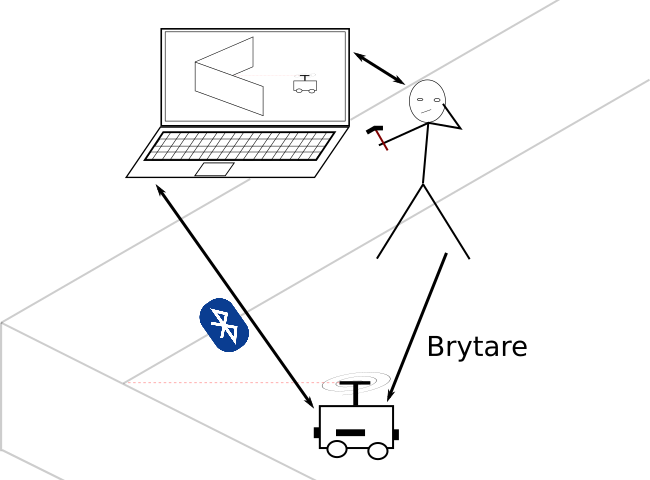
\includegraphics[width=1\textwidth]{overview.png}}
    \caption{Systemet i dess omgivning.}
    \label{fig:overview}
\end{figure}

\newpage
\section{Översikt av systemet}
% TODO: Blockschema, identifiera delsystem och gränssnitt, modularitet och uppgraderbarhet
Systemet är uppbyggt av tre separata moduler, samt en extern PC, enligt figur \ref{fig:modules}. Dessa delsystem kommunicerar med varandra, och med extern hårdvara tillhörande varje modul. Ett mer detaljerat blockschema finns till varje modul, samt i figur \ref{fig:modulesDetailed}.
\begin{figure}[h!]
    \makebox[\textwidth][c]{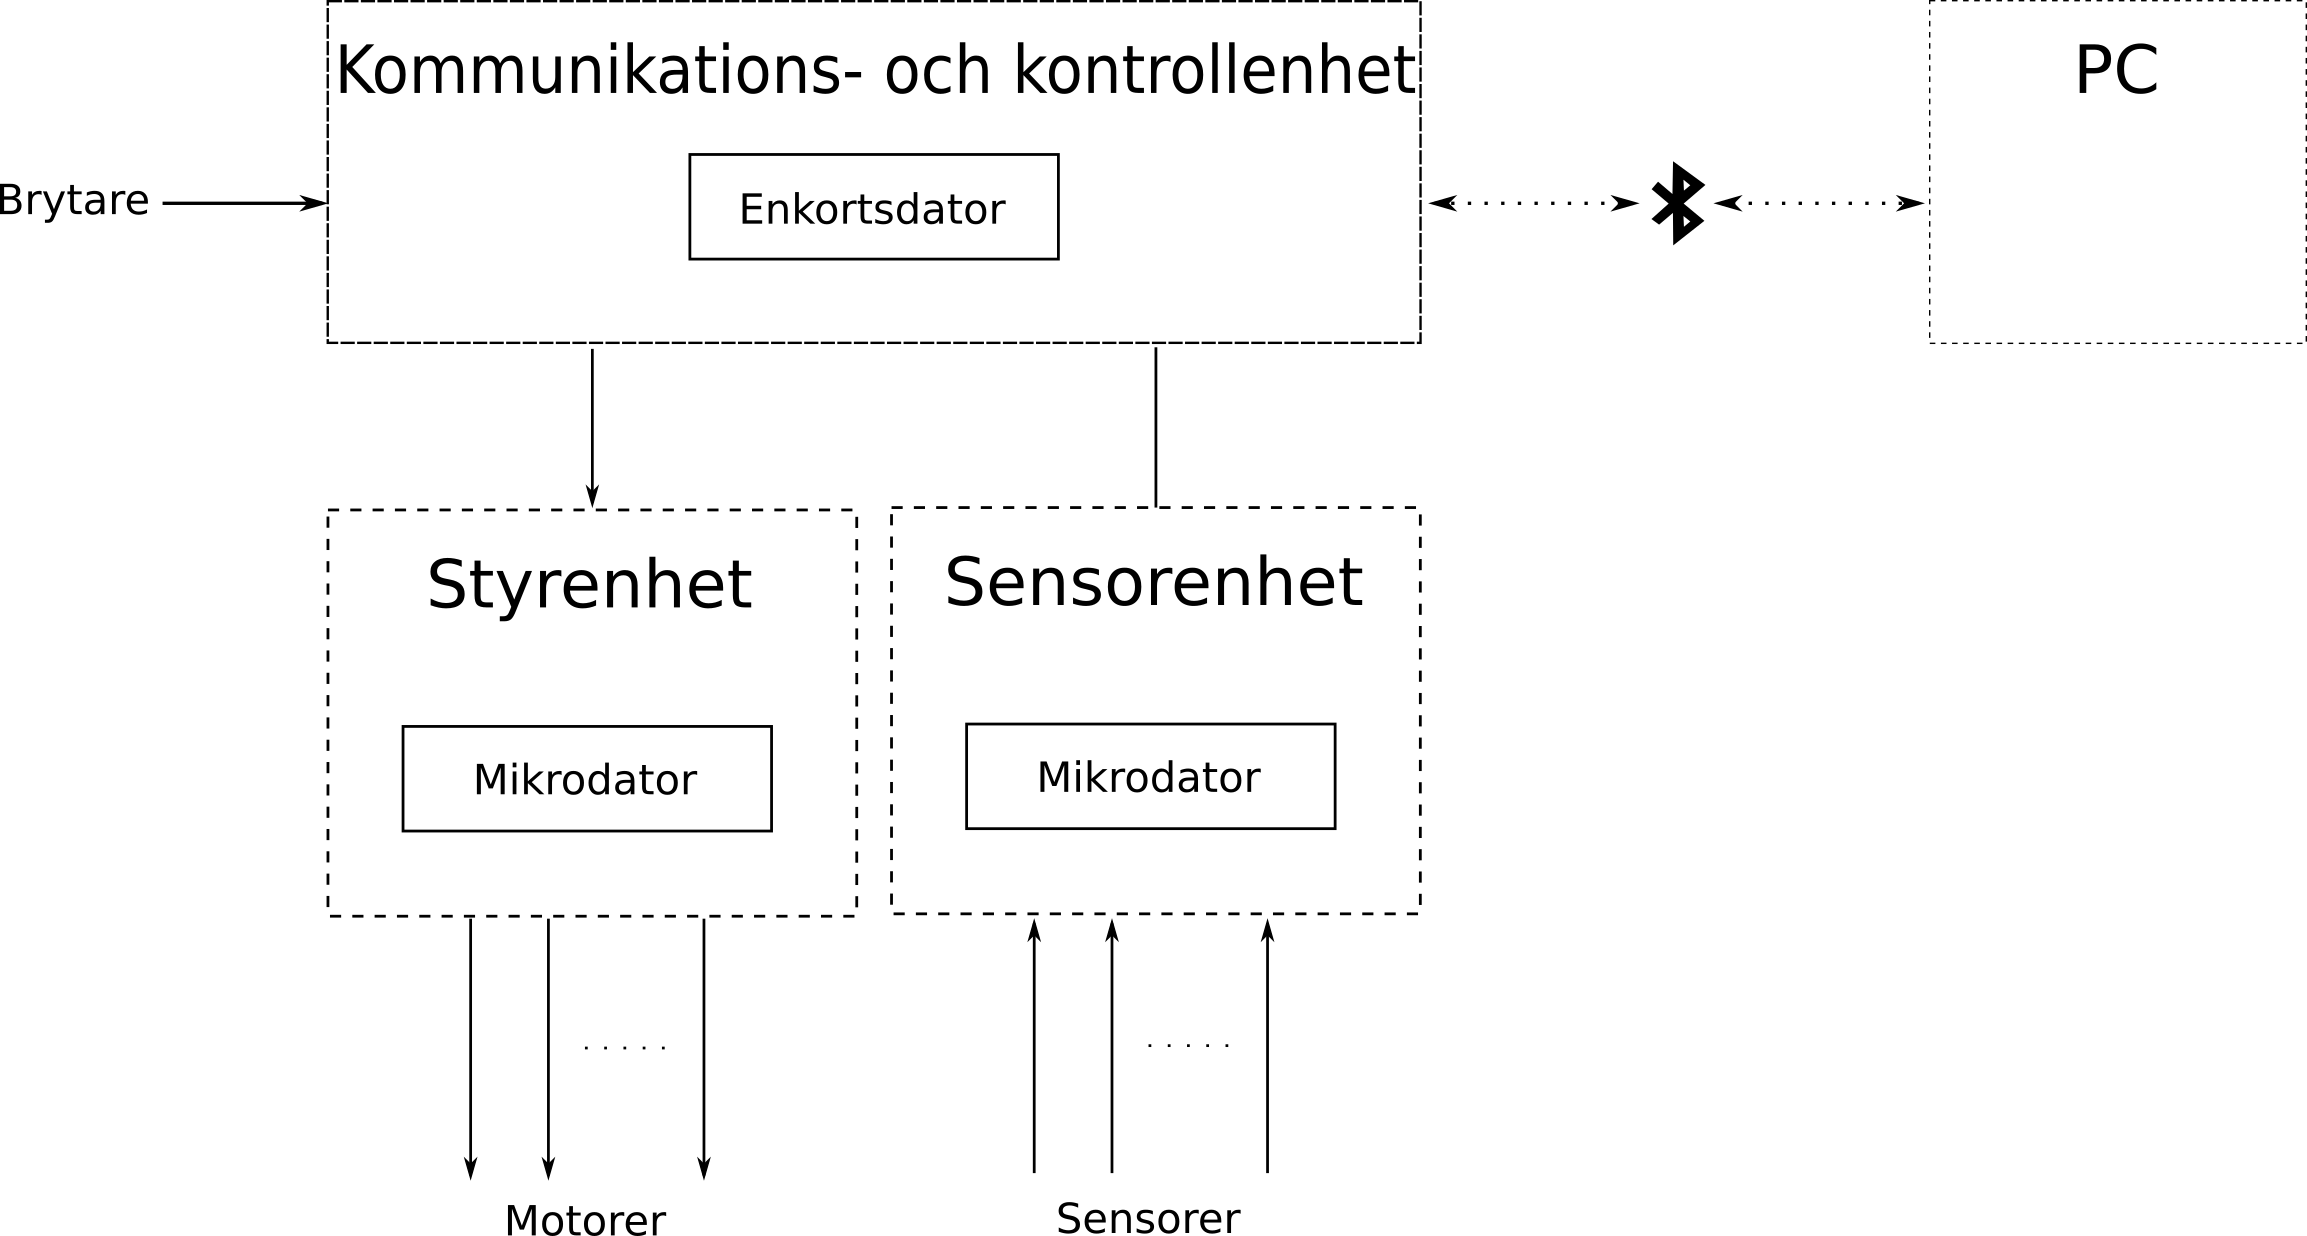
\includegraphics[width=1\textwidth]{modules.png}}
    \caption{Modulöversikt.}
    \label{fig:modules}
\end{figure}

\newpage
\section{Delsystem 1 - Sensorenhet}
% TODO: Ska vi ha en pil till hjärnan? Är väl nån slags tvåvägskommunikation med uart/i2c, även om det inte skickas nån vettig data.
Sensorenheten har i uppgift att läsa in sensordata och omvandla den till ett läsligt format.
\begin{figure}[h!]
    \makebox[\textwidth][c]{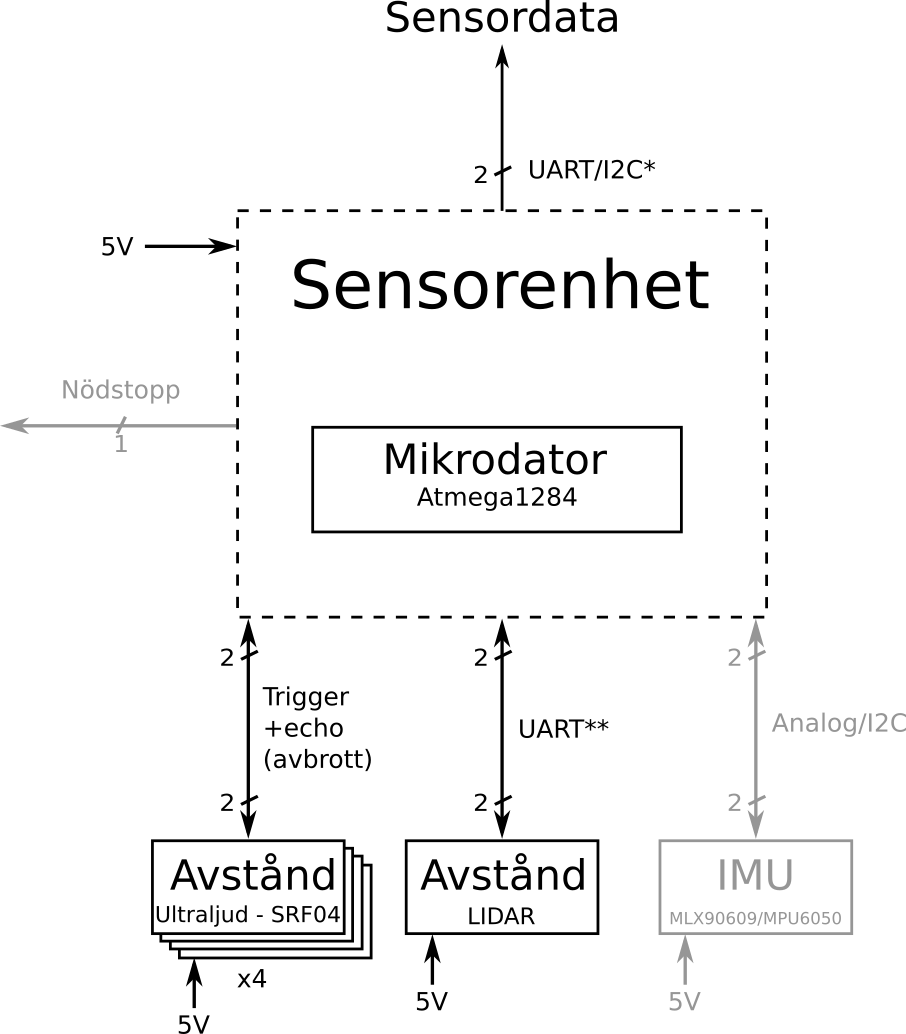
\includegraphics[width=0.6\textwidth]{sensorenhet.png}}
    \caption{Översikt över sensorenheten.}
    \label{fig:modules}
\end{figure}

\noindent \begin{small}
    * Om I\textsuperscript{2}C används krävs även en logic level converter mellan 5V och 3V3 på dessa platser.\\
    ** 5V på Atmega-sidan, 3V3 krävs av sensorn.
\end{small}
\subsection{Hårdvara}

\subsubsection{Processor} %TODO: Minst 4 interrupts, fråga handledare. Kan vi ha flera uarts?

\paragraph{Alternativ 1} % TODO: Är det verkligen 1284-p? Står bara 1284 på föreläsningsbilder.
ATmega1284p används som processormodell, då den både är relativt kraftfull utan att ta det till överdrift, men även har tillräckligt med avbrottsingångar för att kunna arbeta med samtliga ultraljudssensorer, se \ref{sssec:sonicsensors}.

\subsubsection{Ultraljudssensor} \label{sssec:sonicsensors}
En ultraljudssensor, SRF04, placeras på var och en av robotens fyra sidor och används för navigering och positionsuppskattning. Dessa behöver en utgång och en interrupt-ingång var. Se \ref{ssec:sensorInterface}. Dessa kan användas var 65e millisekund utan risk för störningar, vilket ger oss möjlighet att läsa av $\sim15$ sensorer per sekund. Troligtvis kan de även användas med mindre eller ingen marginal, men det kräver testning för att avgöras. %http://www.robot-electronics.co.uk/htm/sonar_faq.htm
% TODO: Alt 2 IRSensor

\subsubsection{LIDAR lite v2} \label{sssec:lidar}
LIDAR är en kraftfull lasersensor som i systemet som helhet används för mätningar som kräver en viss grad av noggranhet. Komponenten kan kommuniceras med via en I\textsuperscript{2}C-buss, som därmed ska användas, se sektion \ref{ssec:sensorInterface}. Processorn behöver mjukvarustöd för detta.

Sensorn monteras på toppen av roboten - ovanpå en roterande servo, som specificeras i större detalj i sektion \ref{ssec:servomotor}. Detta för att effektivt kunna mäta avstånd i flera vinklar.

\subsubsection{IMU} \label{sssec:imu}

\paragraph{Alternativ 1}
En enklare modul, exempelvis MLX90609, används, via en analog ingång. Detta ger oss då endast rotationen kring z-axeln, som kan användas för att beräkna robotens riktning i rummet.

\paragraph{Alternativ 2}
En mer avancerad modul, exempelvis MPU6050, används, via samma I\textsuperscript{2}C-buss som LIDARn. Det ger oss i så fall både riktning och acceleration, för att mer noggrannt kunna beräkna robotens placering. % TODO: MotionMagi, handledare

\subsection{Mjukvara}

Koden ska vara skriven i C, och ska följa <INSERT STANDARD HERE>. Funktioner ska vara kommenterade.

Programmet ska omvandla sensordata till ett mer läsligt format, och ska kunna skicka det vidare (se \ref{ssec:sensorInterface}).

\subsection{Gränssnitt} \label{ssec:sensorInterface}
Sensorenheten kommer behöva kommunicera med de faktiska sensorerna, samt ha ett sätt att passera vidare utdata. Sensorenheten tar inte emot någon indata, och kan inte styras.
%TODO more detailed explenation in general? Specifications around i2c and sonic-sensors output and stuff.
% TODO: A nice picture featuring hardware and interfaces

\subsubsection{LIDAR och gyro}
Då LIDAR lite v2 (\ref{sssec:lidar}) och gyron (\ref{sssec:imu}) kräver en I\textsuperscript{2}C-buss så kommer en sådan att användas för kommunikation mellan dem och processorn. Vi supportar inte flera masters, utan behandlar processorn som den enda, med LIDAR:n och gyron som slavar.

\subsubsection{Ultraljudssensorer}
Ultraljudssensorerna (\ref{sssec:sonicsensors}) är betydligt mer lågnivå i sina gränssnitt, och kommunicerar via spänningsskillnader. Deras utvärde beror på längden på dess höga signal, så för att garantera att vi börjar mäta omedelbart på en hög flank så ska avbrott utnyttjas. Detta uppnås genom att helt enkelt daisy-chaina denna signal till en av avbrottsportarna på processorns

\subsubsection{Utvärden}
Hur passeras processerade mätvärden vidare?

\paragraph{Alternativ 1}
I\textsuperscript{2}C-bussen som användes för att kommunicera med LIDAR:n och gyron kan utnyttjas, med även processorn som slav. Enheten som tar emot data från sensorenheten får istället ta över rollen som master. Se \ref{ssec:brainInterface} för mer detaljer om för och nackdelar.

\paragraph{Alternativ 2}
Implementera en extra UART-buss som endast går mellan sensorenheten och kommunikationsenheten. Se \ref{ssec:brainInterface} för mer detaljer om för och nackdelar.

\newpage
\section{Delsystem 2 - Styrenhet} \label{sec:system2}
\begin{figure}[h!]
    \makebox[\textwidth][c]{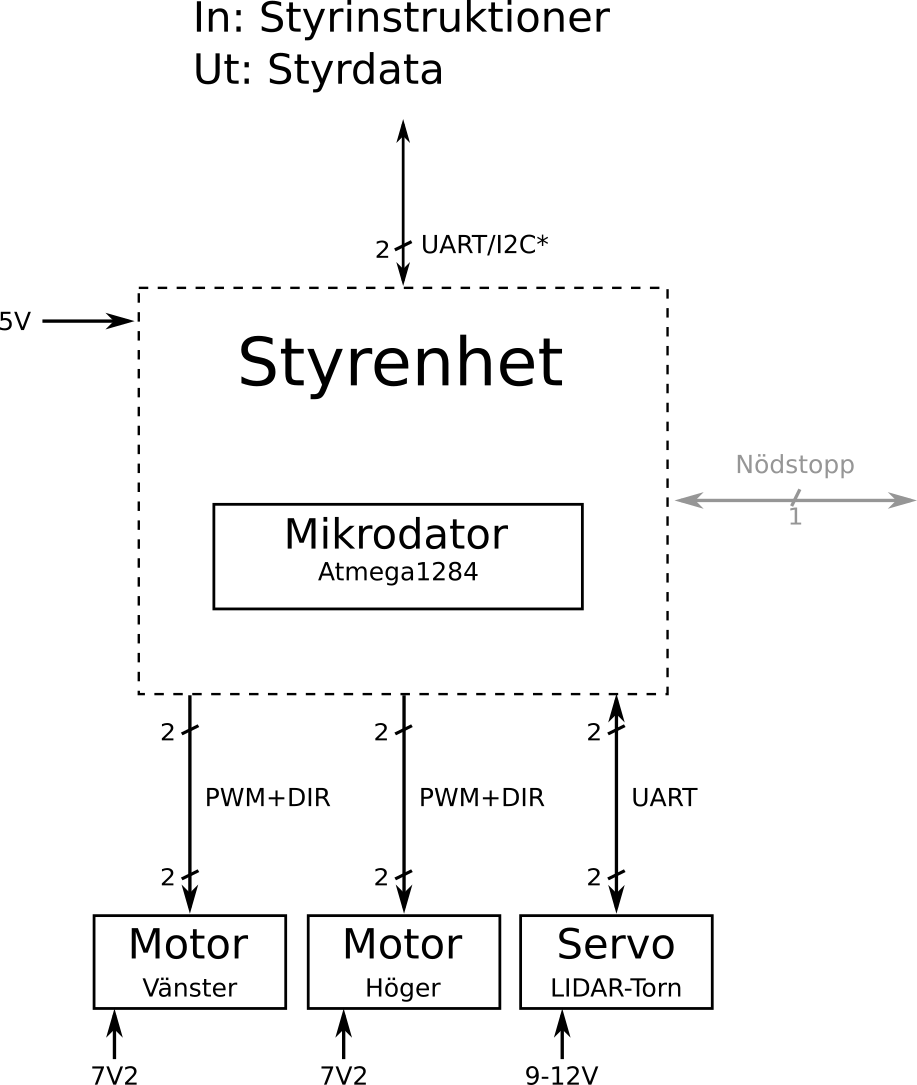
\includegraphics[width=0.6\textwidth]{styrenhet.png}}
    \caption{Översikt över styrenheten.}
    \label{fig:modules}
\end{figure}
\noindent \begin{small}
    * Om I\textsuperscript{2}C används krävs även en logic level converter mellan 5V och 3V3 på dessa platser.
\end{small}
\subsection{Hårdvara}

\subsubsection{Processor}

\paragraph{Alternativ 1}
Processormodellen ATmega1284p.

\paragraph{Alternativ 2}
Processormodellen AtMega1284p's mindre syskon, ATmega16. Denna är inte lika kraftfull som den förstnämnda, men bör definitivt vara kapabel till att utföra dess givna jobb.


\subsubsection{Servo/steppermotor} \label{ssec:servomotor}
På toppen av roboten ska en sensor (se \ref{sssec:lidar}) vara monterad ovanpå en roterande servo, för att tillåta sikt i flera riktningar utan att behöva rotera hela roboten. Typen av servomotor specificeras här.

\paragraph{Alternativ 1}
Servomotorn AX-12 används. Denna har både ett ''vanligt'' läge, och ett så kallat ''wheel''-läge som tillåter fri 360 graders rotation. Det förstnämnda tillåter oss att göra mycket exakta rotationer, men förhindrar oss från att svänga runt ett helt varv. Vi slipper potentiellt felaktiga värden, men kan inte titta rakt bakom oss. Då detta inte är ett stort problem används lämpligen det vanliga läget.
% http://support.robotis.com/en/techsupport_eng.htm#product/dynamixel/ax_series/dxl_ax_actuator.htm
%TODO: AX-12, AX-12A eller AX-12+?
%TODO: Step-up även här?

\subsubsection{Hjulmotorer}
Totalt fyra motorer finns monterade på chassit för hjulstyrning. Detta chassi går under namnet \href{https://docs.isy.liu.se/pub/VanHeden/DataSheets/terminator_prel.pdf}{Terminator}, och de fyra DC-motorerna styrs parvis (höger sida och vänster sida) med hjälp av en PWM-signal samt en rotationsriktningssignal per motorpar.
%TODO: Databladet säger att motorerna jobbar med 7.2V. Är det vad ingångarna tar, eller bara en strömkälla som ligger på sidan? Om det förstnämnda: skriv att vi kräver en step-up krets.

\subsection{Mjukvara}

Koden ska vara skriven i C, och ska följa <INSERT STANDARD HERE>. Funktioner ska vara kommenterade.

\subsection{Gränssnitt} \label{ssec:controllInterface}

\subsubsection{Styrsignaler samt styrdata}

\paragraph{Alternativ 1}
I\textsuperscript{2}C-bussen som användes för sensorer kan användas. Se \ref{ssec:brainInterface} för mer detaljer om för och nackdelar.

\paragraph{Alternativ 2}
Implementera en extra UART-buss som endast går mellan styrenheten och kommunikationsenheten. Se \ref{ssec:brainInterface} för mer detaljer om för och nackdelar.

\newpage
\section{Delsystem 3 - Kommunikations- och kontrollenhet}
\begin{figure}[h!]
    \makebox[\textwidth][c]{
\includegraphics[width=1\textwidth]{brain.png}}
    \caption{Översikt över kommunikations- och kontrollenheten.  }
    \label{fig:modules}
\end{figure}
\noindent \begin{small}
* Om I\textsuperscript{2}C används krävs även en logic level converter mellan 5V och 3V3 på dessa platser.
\end{small}


\subsection{Hårdvara}

\subsubsection{Datormodell}
Då detta delsystem har han om relativt tunga beräkningar används en Raspberry Pi 3. Vi utnyttjar Raspberryns inbyggda blåtand för trådlös kommunikation.

\subsection{Mjukvara}

Koden ska vara skriven i Python 3, och ska följa kodstandarden \href{https://www.python.org/dev/peps/pep-0008/}{PEP 8}.

\subsubsection{Kommunikation}
Delsystemet är vad som i slutändan kontrollerar de olika delsystemen, och måste därför kunna skicka meddelanden mellan de. Den ska ha mjukvara för att kunna skicka meddelanden över de olika gränssnitten som den kopplas upp emot (se \ref{ssec:brainInterface}).

Förutom hårdvarugränssnitt ska den också kunna kommunicera med en extern PC (se \ref{sec:system4}) över blåtand, där den skickar debugdata och kartinformation, och tar emot kommandon vid manuell styrning. Mjukvara för blåtandskommunikation måste finnas.

För att hantera alla dessa meddelanden bör ett meddelandesystem implementeras. Detta görs lämpligen med en prioriterad kö, så att vissa meddelanden kan prioriteras över andra.

\subsubsection{Manuellt läge}
Roboten ska via en brytare kunna byta mellan ett autonomt och ett manuellt läge. I det manuella ska den ta emot kommandon från PC:n via blåtand (se \ref{sec:system4}) om hur den ska åka, mycket likt en radiostyrd bil. Mjukvara för att på ett korrekt sätt utföra dessa kommandon behövs.

\subsubsection{Kartritning}
Robotens huvuduppdrag i det autonoma läget är att skanna ett rum och rita en karta över det. Mjukvara för att omvandla skannerdata till ett tvådimensionellt rum, samt rutiner för att söka upp och skanna outforskade delar av rummet ska finnas.

\subsubsection{Ruttstyrning}
Roboten behöver kontinuerligt ta och leta sig till outfoskade delar av rummet i det autonoma läget. En algoritm för att hitta ett lämpligt outforskat ställe, en för att hitta en väg dit, och en som skickar korrekta meddelanden till styrenheten (se \ref{sec:system2}) för att ta sig dit behövs.

\subsection{Gränssnitt} \label{ssec:brainInterface}

\paragraph{Alternativ 1}
I\textsuperscript{2}C via samma buss som sensorer, där kommunikationsenheten agerar master. Detta gör att vi slipper implementera UART, men gör att både sensorer och tre moduler behöver samsas på samma buss. Har även nackdelen att kod i kommunikationsenheten behöver modifieras när sensoruppsättningen förändras, vilket minskar modulariteten. %TODO: Visst behöver mastern styra alla inkopplade enheter?
Vid kommunikationsenheten behöver dessutom en logic level shifter användas, då Raspberry Pi använder 3v3 och övriga moduler 5v.

\paragraph{Alternativ 2}
Som alternativ till I\textsuperscript{2}C kan UART användas. Raspberry Pi 3 har ingen inbyggd UART kan användas utan bland annat låsa klockfrekvensen och använda spänningsomvandlare från 5v till 3v3, och har dessutom bara en ledig om blåtand används samtidigt. Istället kan två 5 volts-kompatibla USB till UART-moduler, exempelvis CH340G, användas. Nackdelen är att även UART måste implementeras, vilket dock verkar relativt trivialt. % TODO: LiU har förmodligen inte samma saker som kina (https://www.aliexpress.com/item/CH340-Serial-Converter-USB-To-TTL-6PIN-Module-Upgrade-Small-Plate-for-PRO-mini-Instead-of/1856263846.html). CP2102 kanske (om den är 5v-kompatibel).

\newpage
\section{Delsystem 4 - Mjukvara på PC} \label{sec:system4}
\begin{figure}[h!]
    \makebox[\textwidth][c]{
\includegraphics[width=0.4\textwidth]{PC.png}}
    \caption{Översikt över PCn.}
    \label{fig:modules}
\end{figure}
\subsection{Hårdvara}
En PC med tangentbord, mus, skärm och blåtandsmodul.

\subsection{Mjukvara}

Koden ska vara skriven i Python 3, och ska följa kodstandarden \href{https://www.python.org/dev/peps/pep-0008/}{PEP 8}.

\subsubsection{Input}
PC-mjukvaran tar emot sensor, styrdata och kartdata från kommunikationsenheten via blåtand. Den tar också emot instruktioner från mus och tangentbord. 

\subsubsection{Output}
Mjukvaran skickar styrkommandon samt uppmaning om att läsa av sensorerna till roboten i dess manuella läge. Den kan också skicka kommandon om att växla mellan autonomt och manuellt läge, som då går före den fysiska brytaren på roboten.

Informationen som tas emot från roboten presenteras i ett grafiskt gränssnitt.

\subsection{Gränssnitt} \label{ssec:PCInterface}

\newpage
\begin{appendices}
\chapter{Detaljerat blockschema}
\\% TODO: Riktig titel
\begin{figure}[h!]
    \makebox[\textwidth][c]{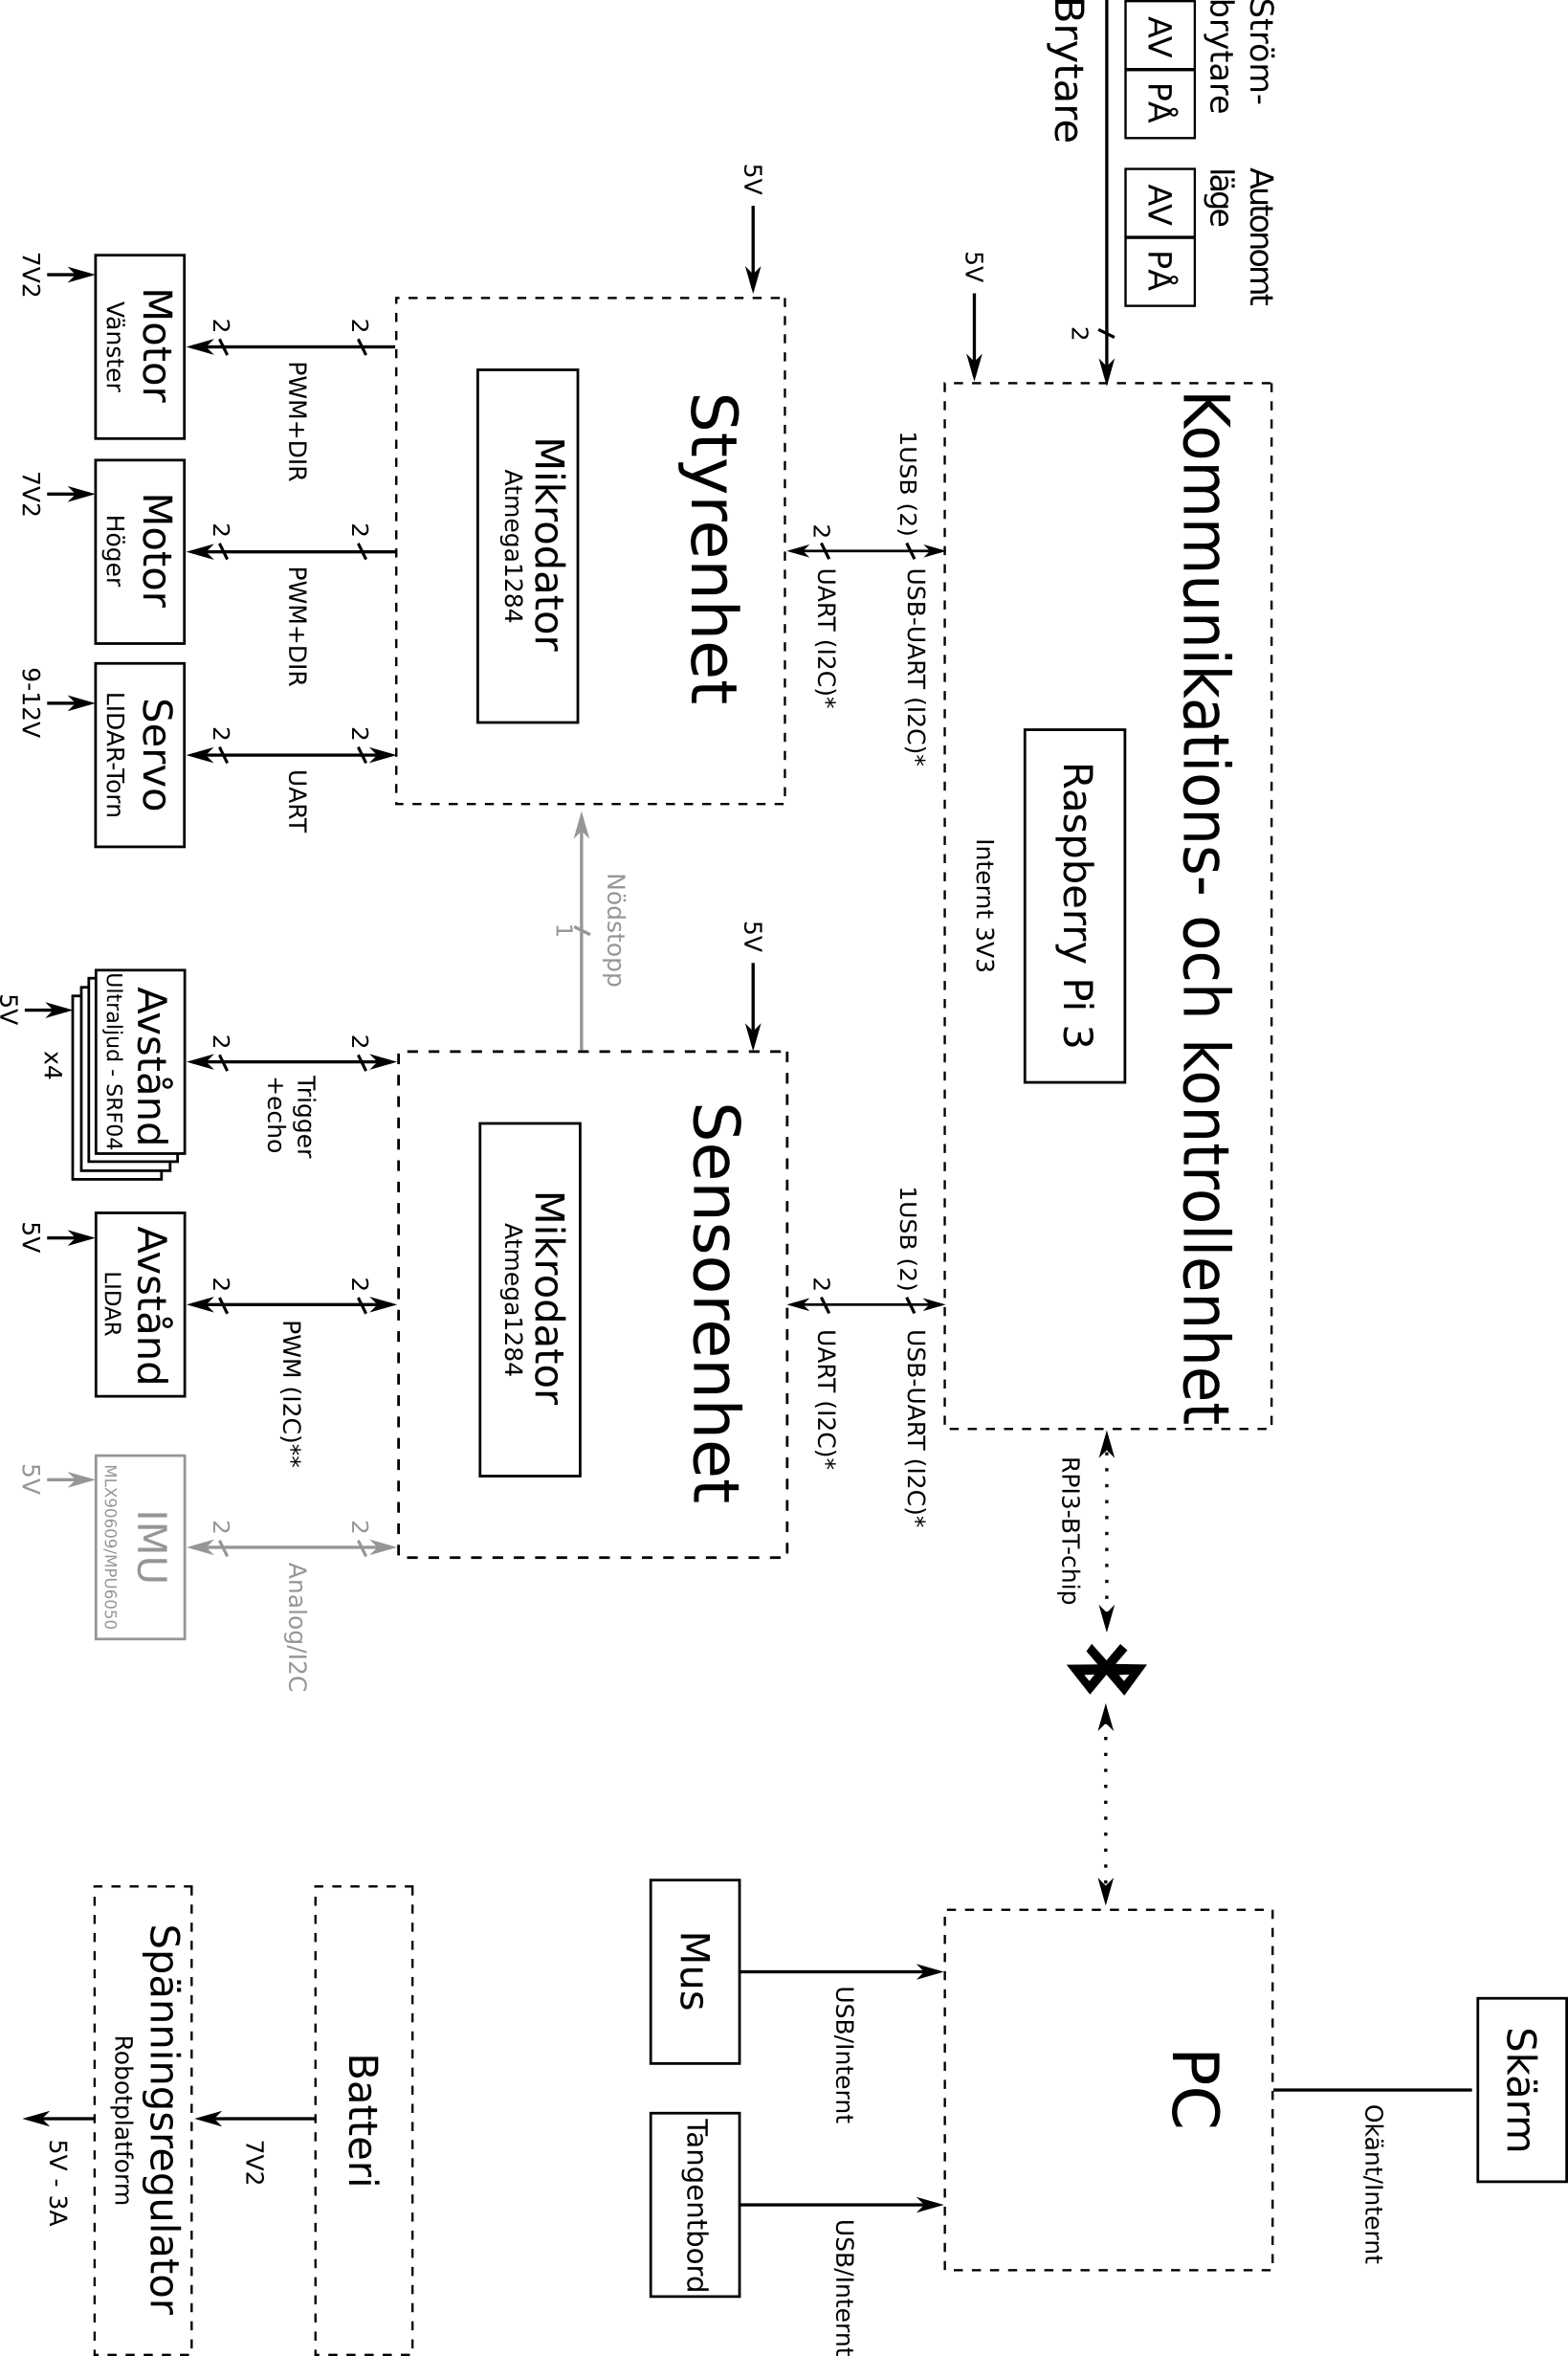
\includegraphics[width=0.85\textwidth]{modules_detail.png}}
    \caption{Detaljerat blockschema över systemet.}
    \label{fig:modulesDetailed}
\end{figure}
* Om I\textsuperscript{2}C används krävs även en logic level converter mellan 5V och 3V3 på dessa platser.\\
** 5V på Atmega-sidan, 3V3 krävs av sensorn.

\end{appendices}


\end{document}
